\emph{Feature subset and adaptation without target labels.} Table~\ref{tab:arms} tests whether other inputs or adaptation methods close the gap. Restricting the models to the nine exporter-robust columns raises held-out source balanced accuracy for five architectures but lowers it for LR (\RArmRobLRSrc{} against \RArmPlainLRSrc). On the clean target flows, XGB and HGB keep their level (\RArmRobXGBClean{} and \RArmRobHGBClean), whereas DT and RF fall to \RArmRobDTClean{} and \RArmRobRFClean: the columns that an exporter moves least are not enough. None of the three adaptation methods that read unlabeled target flows beats the plain tree-based models. Importance weighting changes little (\RArmIwTreeCleanMin{} to \RArmIwTreeCleanMax{} for the tree-based models), because its domain classifier separates the corpora so well that the weights concentrate on \RIwESSmin\% to \RIwESSmax\% of the source flows in effective sample size. CORAL raises the MLP from \RArmPlainMLPClean{} to \RArmCoralMLPClean{} but pushes the target false positive rate of the tree-based models to \RArmCoralTreeFPRmin{} to \RArmCoralTreeFPRmax, as in our first analysis. Domain-adversarial training reaches \RArmDannDANNClean.

\begin{table}[t]
\caption{Transfer from \DA{} to \DB{} under other feature sets and with adaptation, mean over 20 splits, at $\tau = 0.5$. Importance weighting, CORAL, and DANN read unlabeled target flows. Clean: the benign-labeled copies removed; relab.: the copies labeled as attack.}
\label{tab:arms}
\centering
\scriptsize
\setlength{\tabcolsep}{2.6pt}
\begin{tabular}{llccccc}
\toprule
Arm & Model & Src.\ BA & \multicolumn{3}{c}{Target, clean} & Target, relab. \\
\cmidrule(lr){4-6}
 & & & BA & AUC & FPR & BA \\
\midrule
Shared space (18) & LR & 0.837 & 0.613 & 0.796 & 0.061 & 0.574 \\
 & DT & 0.822 & 0.781 & 0.783 & 0.206 & 0.802 \\
 & RF & 0.808 & 0.818 & 0.879 & 0.232 & 0.836 \\
 & XGB & 0.865 & 0.858 & 0.896 & 0.083 & 0.886 \\
 & HGB & 0.867 & 0.860 & 0.888 & 0.064 & 0.890 \\
 & MLP & 0.903 & 0.688 & 0.806 & 0.432 & 0.715 \\
\midrule
Exporter-robust (9) & LR & 0.804 & 0.615 & 0.821 & 0.646 & 0.632 \\
 & DT & 0.883 & 0.616 & 0.633 & 0.546 & 0.647 \\
 & RF & 0.894 & 0.599 & 0.781 & 0.578 & 0.630 \\
 & XGB & 0.925 & 0.835 & 0.847 & 0.076 & 0.870 \\
 & HGB & 0.939 & 0.837 & 0.860 & 0.082 & 0.871 \\
 & MLP & 0.937 & 0.651 & 0.815 & 0.479 & 0.681 \\
\midrule
Importance weighting & LR & 0.696 & 0.624 & 0.789 & 0.533 & 0.630 \\
 & DT & 0.831 & 0.782 & 0.754 & 0.167 & 0.802 \\
 & RF & 0.788 & 0.812 & 0.878 & 0.223 & 0.830 \\
 & XGB & 0.831 & 0.837 & 0.882 & 0.103 & 0.858 \\
 & HGB & 0.814 & 0.740 & 0.863 & 0.220 & 0.768 \\
 & MLP & 0.842 & 0.684 & 0.795 & 0.438 & 0.707 \\
\midrule
CORAL & LR & 0.836 & 0.585 & 0.855 & 0.741 & 0.597 \\
 & DT & 0.818 & 0.539 & 0.543 & 0.794 & 0.546 \\
 & RF & 0.805 & 0.482 & 0.761 & 0.985 & 0.489 \\
 & XGB & 0.903 & 0.539 & 0.736 & 0.766 & 0.560 \\
 & HGB & 0.891 & 0.521 & 0.741 & 0.820 & 0.536 \\
 & MLP & 0.932 & 0.813 & 0.815 & 0.177 & 0.825 \\
\midrule
DANN & DANN & 0.895 & 0.655 & 0.814 & 0.600 & 0.661 \\
\bottomrule
\end{tabular}

\end{table}

\emph{A few labeled target captures.} Labeled data from the target helps far more (Fig.~\ref{fig:labeleff}). Added to the \DA{} training data, a single labeled capture file of \DB{} raises the balanced accuracy of the five nonlinear architectures on the capture files not drawn to \RLeSrcOneNlMin{} to \RLeSrcOneNlMax{} (the MLP from \RLeZeroMLP{} to \RLeSrcOneMLP), close to the leave-one-capture-file-out reference, and eight files to \RLeSrcEightNlMin{} to \RLeSrcEightNlMax. The same capture files alone give only \RLeTgtOneNlMin{} to \RLeTgtOneNlMax{} for one file, so the source data still carries most of what the detectors know. The alert bound takes more data. With the threshold fixed on source data, the six architectures met all three alert conditions in \RLeSrcOneMeet{} of \RLeSrcOneCells{} draws with one labeled file and in \RLeSrcEightMeet{} of \RLeSrcEightCells{} with eight; with eight files, XGB and the MLP met them in every draw, at \RLeSrcEightXGBAlerts{} and \RLeSrcEightMLPAlerts{} false alerts per hour on average and a recall of about \RLeSrcEightXGBRecall.

\begin{figure*}[t]
\centering
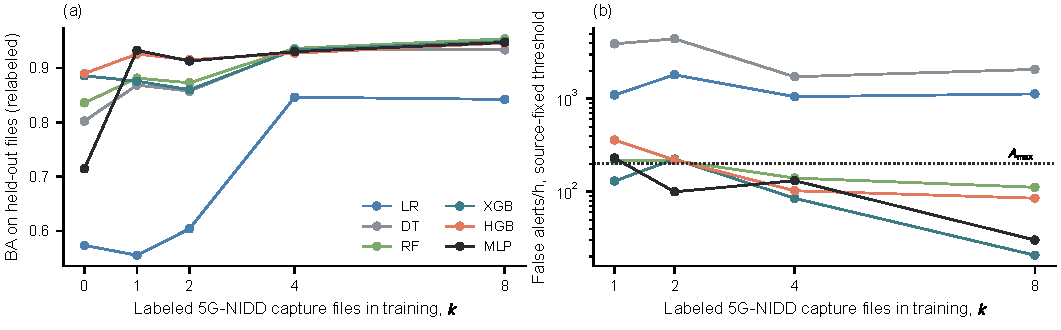
\includegraphics[width=0.92\textwidth]{figs/fig_label_efficient}
\caption{Label-efficient arm: $k$ labeled capture files of \DB{} added to the \DA{} training data (four random draws per $k$; $k = 0$ is the plain transfer of the 20 splits), evaluated on the capture files not drawn, with the copies relabeled as attack. (a) Balanced accuracy; (b) false alerts per hour at the threshold fixed on source data, mean over draws, with the bound $A_{\max}$.}
\label{fig:labeleff}
\end{figure*}

\emph{Size of the source sample.} Repeating the transfer with \RSzNlist{} source flows (\RSzSplits{} splits, five architectures) changed clean target balanced accuracy by at most \RSzMaxChangeClean{} against \NSub{} flows, in no consistent direction, which is within the variation between splits.
